\documentclass[a4paper, spanish]{article}

\usepackage[T1]{fontenc}
\usepackage[utf8]{inputenc}
\usepackage{babel, parskip}
\usepackage[colorlinks]{hyperref}
\usepackage{graphicx}


\title{Projectizer Delux Pro XP \\ Documento de Diseño del Sistema SAR}
\author{Version 1.0 \\ M. Blanc, L.C. Jariego, P. Marcos, F. Martín, D. Nevado}

\begin{document}


\maketitle
\begin{abstract}
Simpatico resumen aqui.
\end{abstract}
\vspace{\fill}
\tableofcontents
%% Estas dos lineas son temporales
%\pagebreak
\let\oldsection\section\renewcommand\section{\clearpage\oldsection}

\section{Descripción de la Arquitectura del Sistema}
La arquitectura de este sistema informático se basa en un patrón MVC (Modelo Vista Controlador). La idea fundamental de este patrón es separa la interfaz

Aquí el equipo debe describir brevemente en qué consiste este patrón.
 
Describir las clases y enumeraciones del diagrama de clases que se realiza en el apartado 2 de este documento.

\section{Diagrama de Clases}
\begin{figure}[h!]
\centering
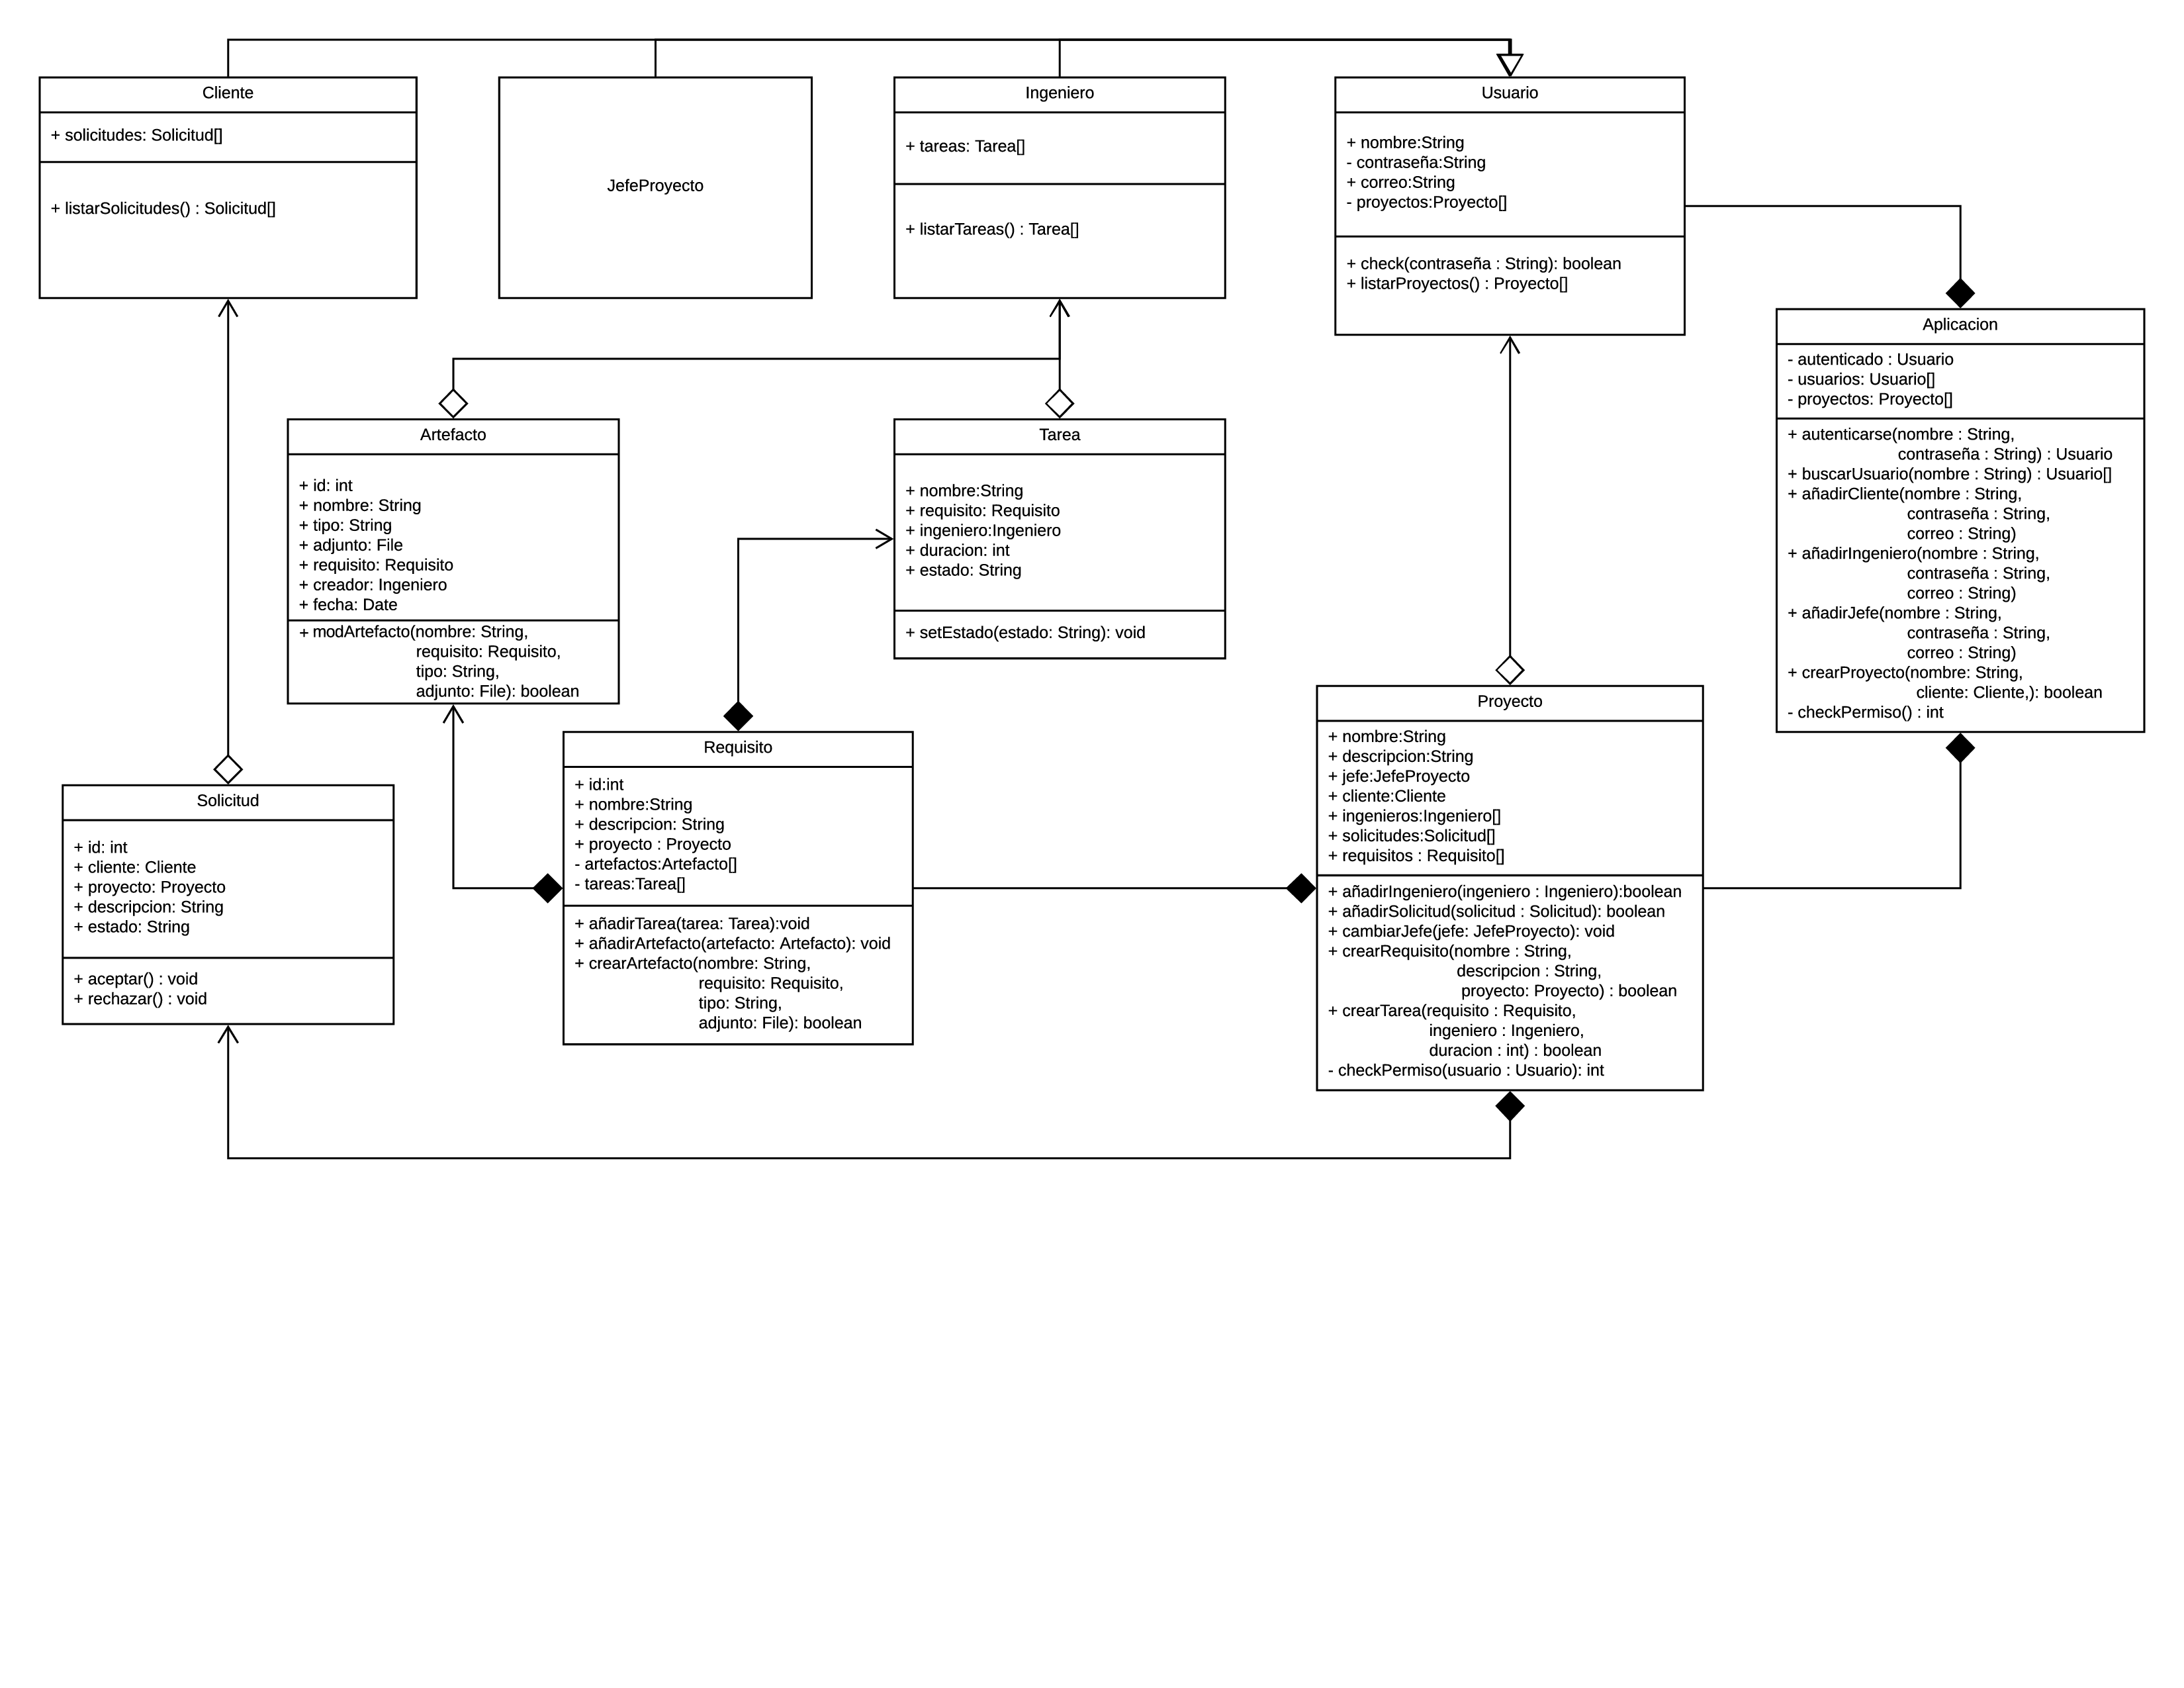
\includegraphics[width=0.9\textwidth]{diagramas/diagrama-clases.png}
\caption{Diagrama de clases}
\end{figure}

\section{Diagramas de Secuencia}
Según UML los argumentos son opcionales.
Hemos decidido no incluirlos para no sobrecargar el diagrama y transmitir mejor el mensaje.

\subsection{Especificar Requisito} % Diagrama de secuencia obligatorio num 1
\begin{figure}[h!]
\centering
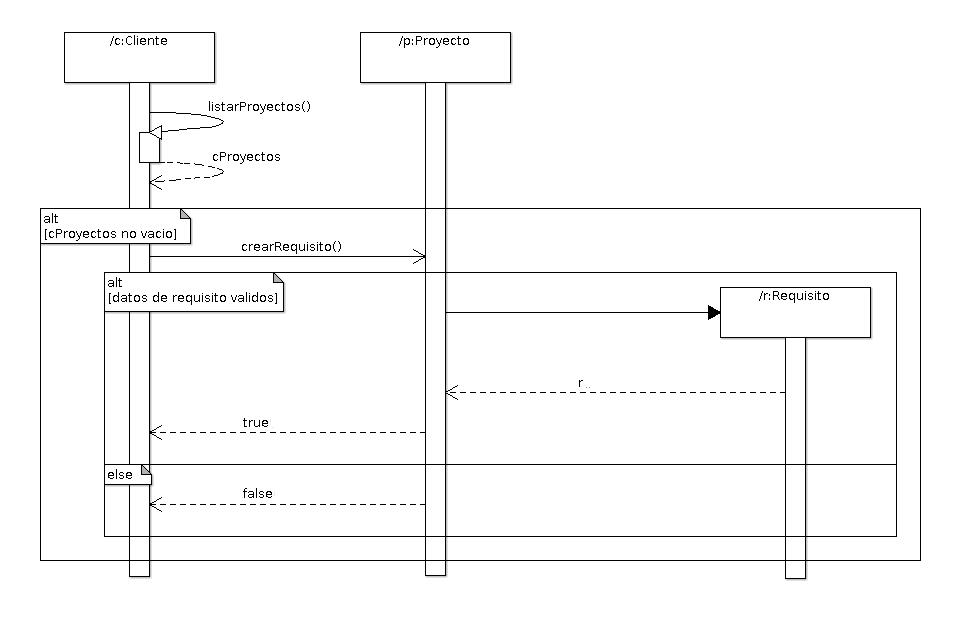
\includegraphics[width=0.9\textwidth]{diagramas/diagramasSecuencia/CrearRequisito_sd.png}
\caption{Diagrama de secuencia para CrearRequisitos}
\end{figure}


\subsection{Crear Proyecto} % Diagrama de secuencia obligatorio num 2
\begin{figure}[h!]
\centering
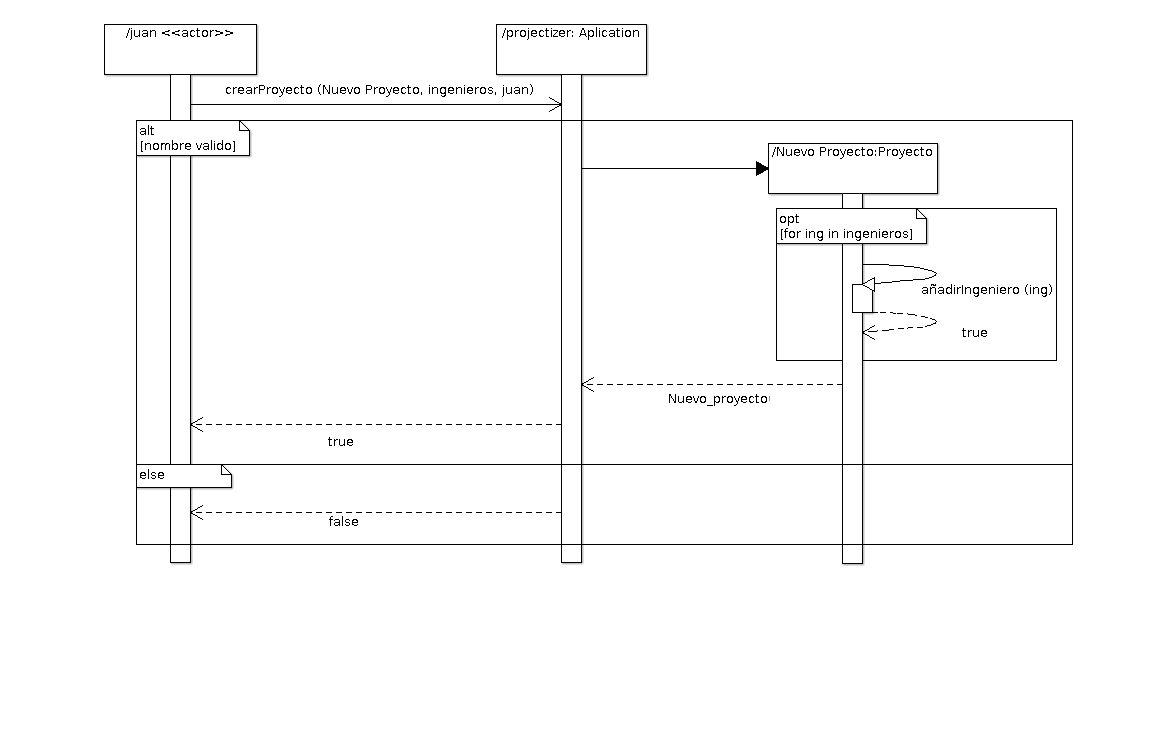
\includegraphics[width=0.9\textwidth]{diagramas/diagramasSecuencia/CrearProyecto_sd.png}
\caption{Diagrama de secuencia para CrearProyecto}
\end{figure}


\subsection{Crear Solicitud de Requisito} % Diagrama de secuencia obligatorio num 3
\begin{figure}[h!]
\centering
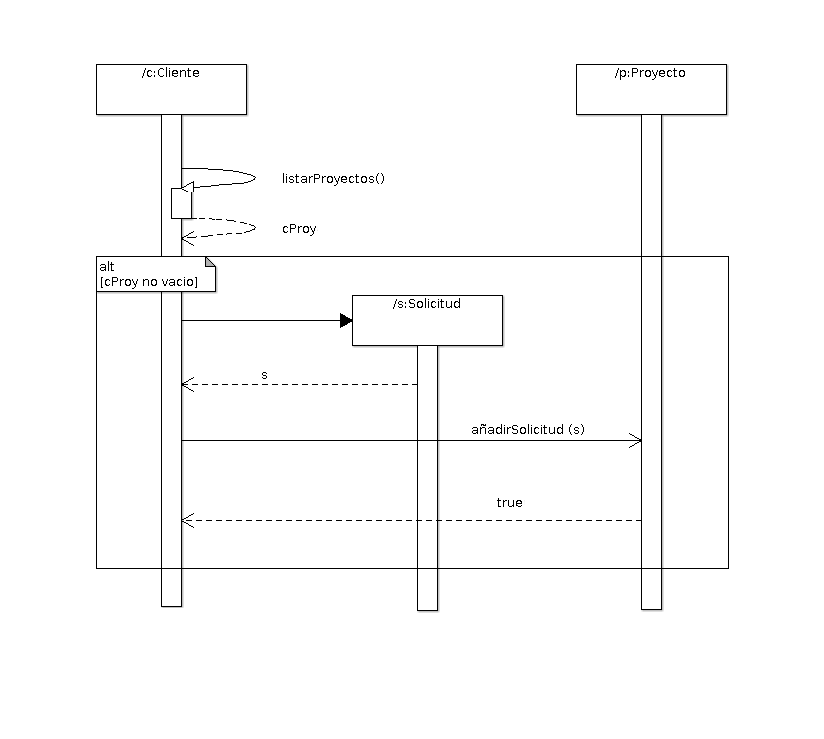
\includegraphics[width=0.9\textwidth]{diagramas/diagramasSecuencia/CrearSolicitud_sd.png}
\caption{Diagrama de secuencia para CrearSolicitud}
\end{figure}


\subsection{Crear Artefacto}
\begin{figure}[h!]
\centering
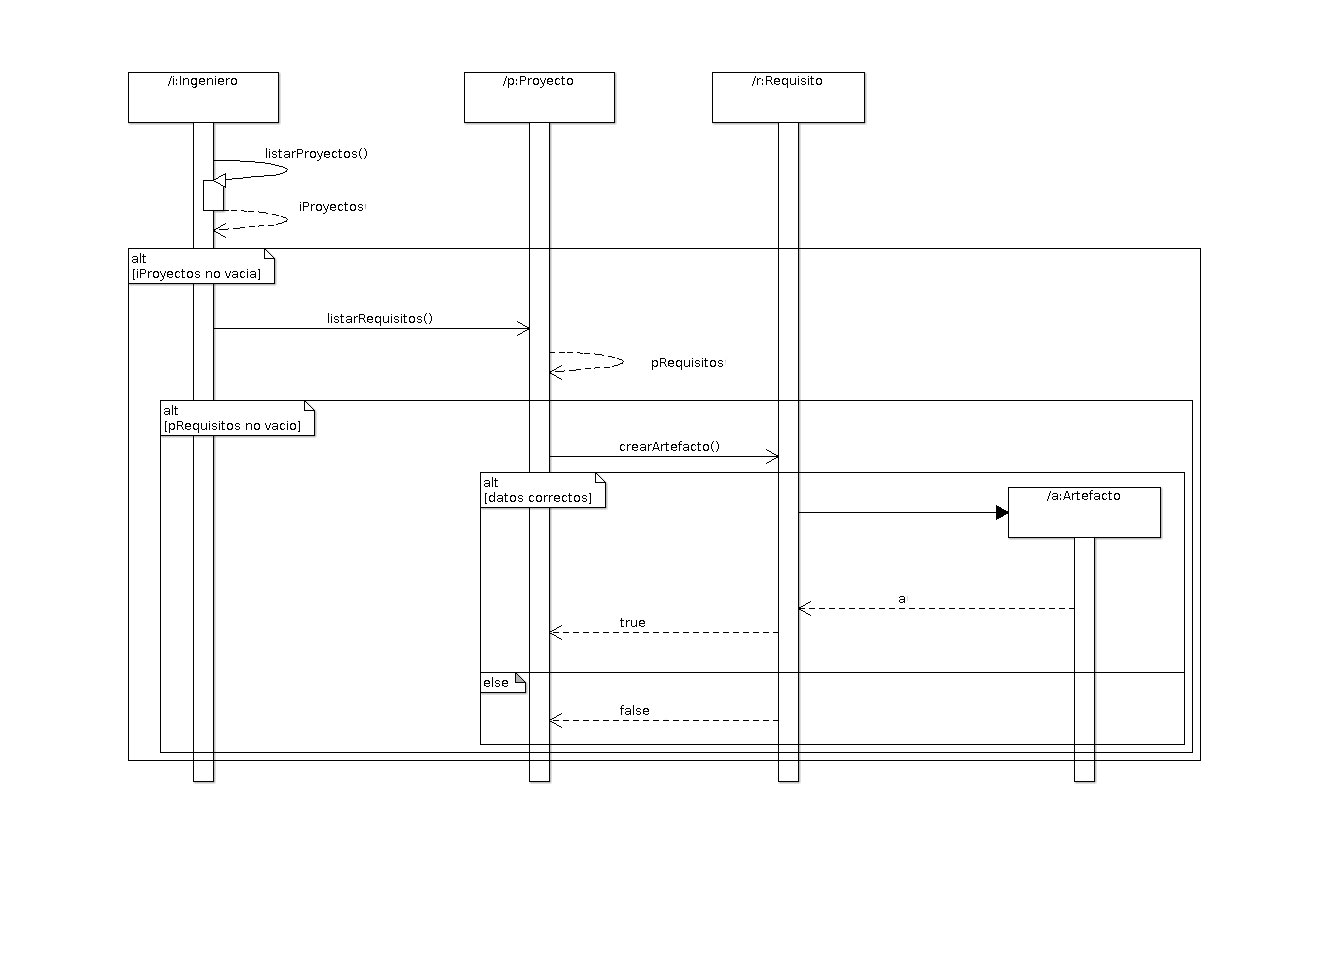
\includegraphics[width=0.9\textwidth]{diagramas/diagramasSecuencia/CrearArtefacto_sd.png}
\caption{Diagrama de secuencia para CrearArtefacto}
\end{figure}

\section{Glosario}
\begin{description}
  \item [SAR] Abreviación de Sistema de Análisis de Requisitos
  \item [JdP] Abreviación de Jefe de Proyecto
  \item [Solicitud] Solicitud de un requisito nuevo
  \item [Artefacto] Un producto tangible producido durante el desarrollo.
  \item [Scrum] Metodología de desarrollo ágil comercial. 
\end{description}

\end{document}